\newpage

\section{Fuzzy variables}

Three linguistic variables have been selected for input, based on the sensor readings of the saucer:

\begin{itemize}
	\item Distance to target
	\item Energy difference
	\item Heading angle
\end{itemize}

\subsection{Distance to target}

Distance to target is the distance from the saucer to the opponent, and is measured in meters. The universe of disclosure for distance is between 0 meters and the diagonal length of the battle space. The formula has been supplied in the existing code as:
\\
\\
$\sqrt{\mbox{width} \cdot \mbox{width} + \mbox{height} \cdot \mbox{height}}$
\\
\\
This linguistic variable is used to determine how much energy will be committed to firing the cannon. As mentioned previously, the cannon will only be fired at close or near distances. Therefore, three fuzzy sets are associated with distance:

\begin{figure}[H]
\centering
\caption{Distance to target fuzzy sets}
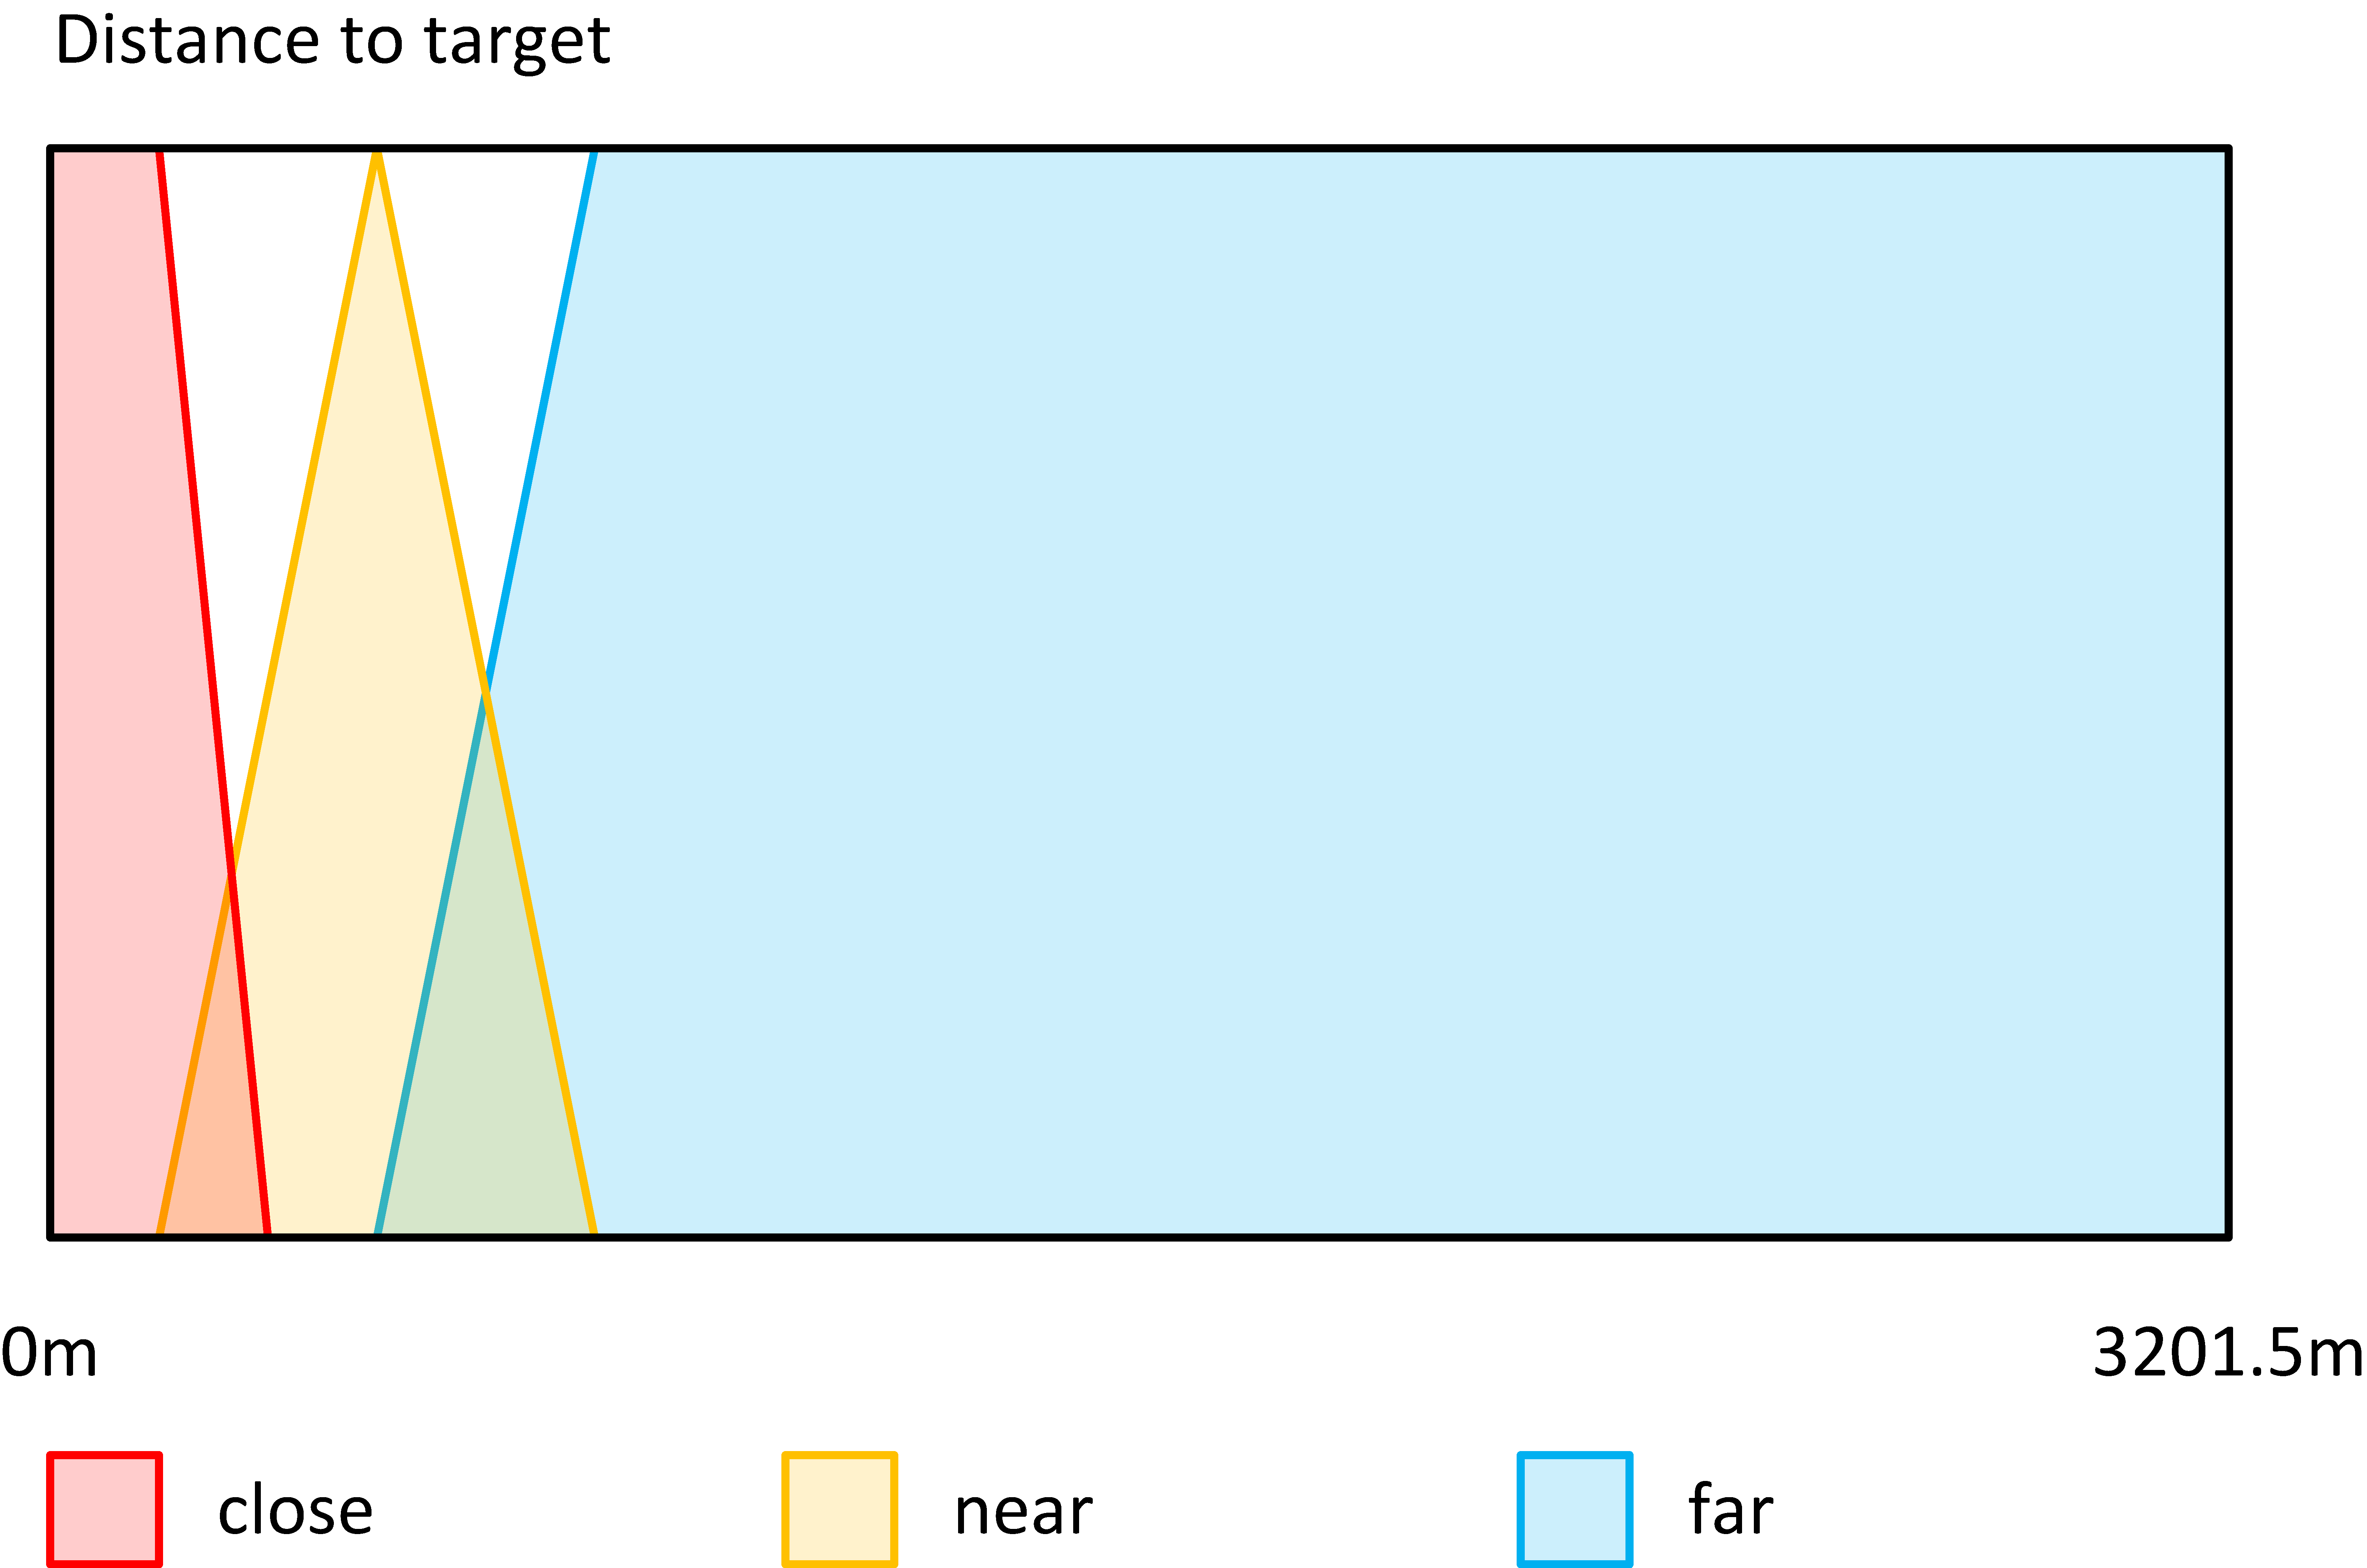
\includegraphics[scale=0.1]{./img/pdf/distanceSets.pdf}
\end{figure}

\subsection{Energy difference}

Energy difference is the difference between the saucer's energy and the opponent's energy. The universe of disclosure for energyDifference is between -10,000j to +10,000j, where 10,000j is the amount of energy that the saucers begin with. This linguistic variable determines who is winning, who is losing, or if the score is even. It is used as input to decide how much energy is committed in firing the weapon, as well as whether or not to turn into or away from the enemy. The following fuzzy sets are created for energy difference:

\begin{figure}[H]
\centering
\caption{Energy difference fuzzy sets}
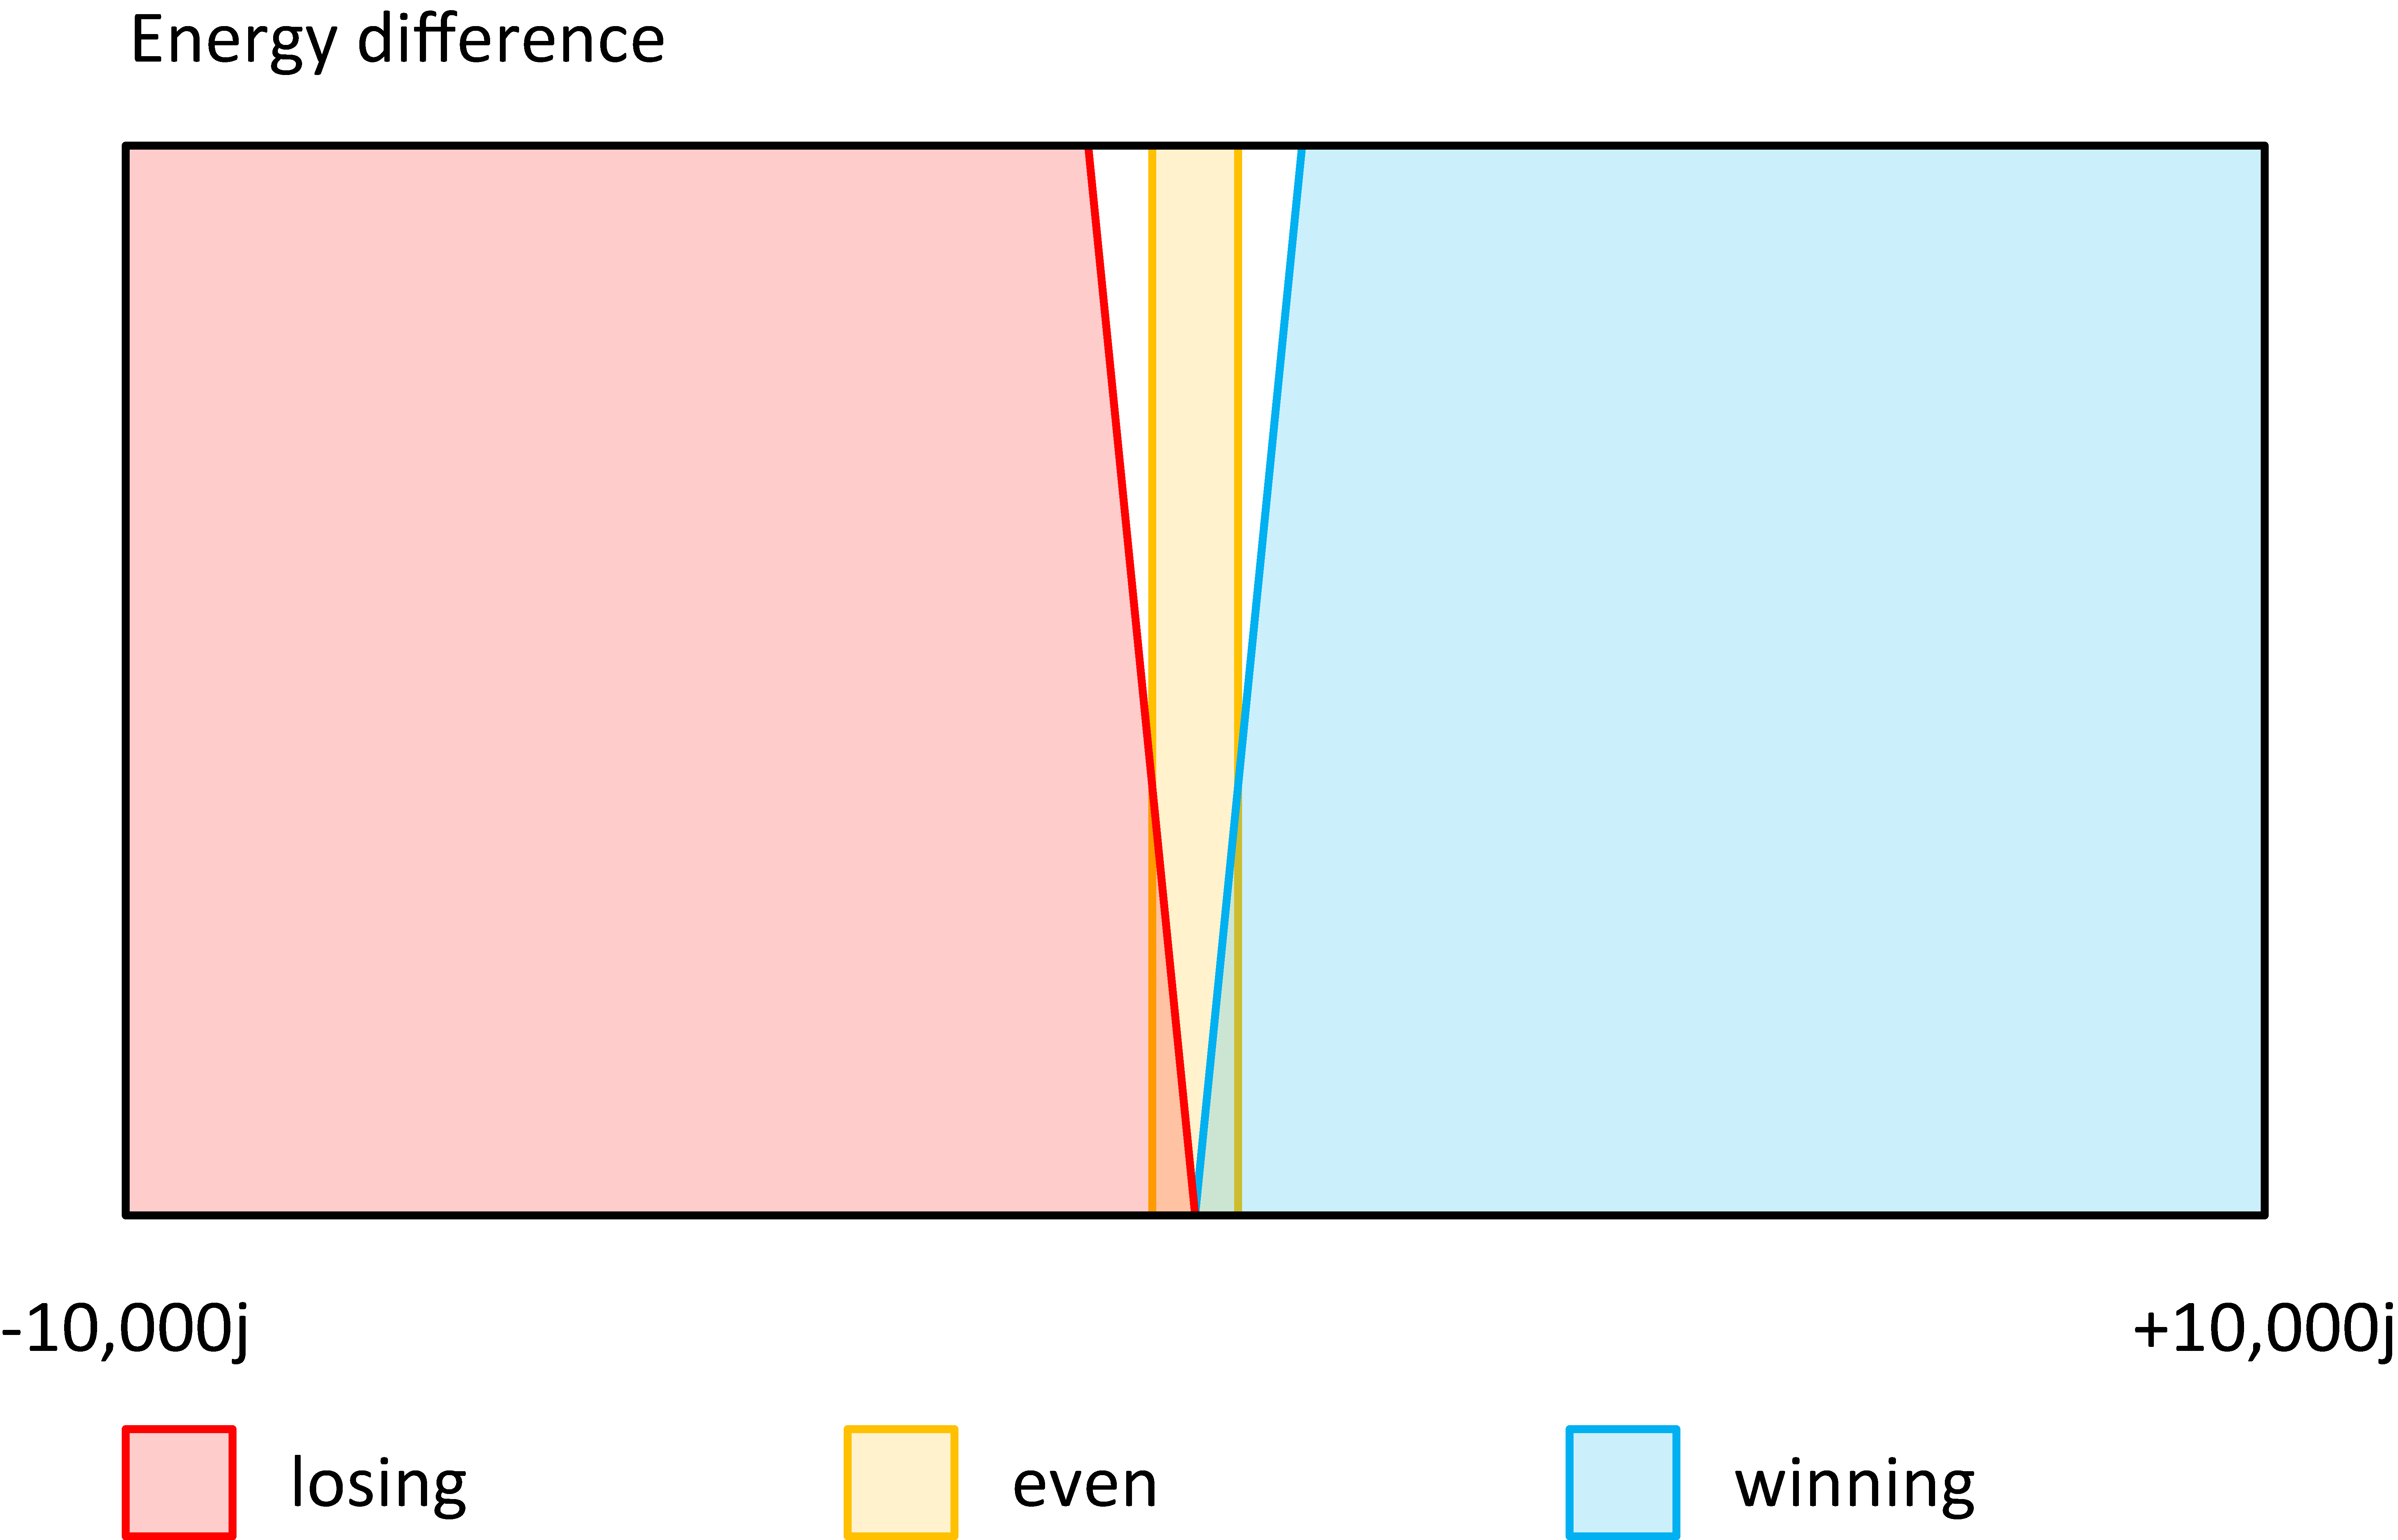
\includegraphics[scale=0.1]{./img/pdf/energyDiffSets.pdf}
\end{figure}

\subsection{Heading angle}

Heading angle is the direction of the opponent in relation to the saucer, in degrees. After printing \mintinline{java}{opponentDirection} during execution, it is assumed that the universe of disclosure for this linguistic variable is from -360$^{\circ}$ to +360$^{\circ}$. The variable, in conjunction with energy difference, dictates how the saucer will turn, and has been configured with the following fuzzy sets:

\begin{itemize}
	\item rearRight
	\item hardRight
	\item right
	\item smallRight
	\item straightAhead
	\item smallLeft
	\item left
	\item hardleft
	\item rearLeft
\end{itemize}